\label{sec:setting-survey}

\noindent As mentioned in the introduction, the setting for this thesis is Hawassa Industrial Park (HIP), a special economic zone in Southern Ethiopia. The Park hosts foreign-owned garment and textile firms\footnote{Mostly Chinese and Indian. The Park was built by the Chinese construction giant China Civil Engineering Construction Corporation, involved in a number of other projects in Africa, in 2016.}, operating under government incentive schemes. Production is exclusively for export. Nonetheless, factory jobs at HIP pay little by local standards and demand eight-hour shifts, six days a week \citep{agarwal2026fieldnotes}. \\
\smallskip

\parhead{Data structure}

\noindent I use administrative data on firms present in HIP, and survey data on their employees. Both come from the baseline of a forthcoming project by Agarwal, Grosset-Touba and Wu, fielded between April and June 2026. Please note that I am operating with a restricted, cross-sectional version of the survey\footnote{This thesis was written during Wave 1, and before Wave 2 was run.}.\\

\noindent As mentioned in the introduction, the survey presents three remarkable features:
\begin{enumerate}
    \item \textit{It captures the beginning of the network.} \\
    In a standing network, every tie was formed at some unrecorded moment and has survived since. The econometrician sees a stock, and cannot tell a tie made inside the institution from one brought to it. Here, workers are interviewed shortly after being hired, and are explicitely asked if their ties predates that hire or not. 
    \item  \textit{It captures the choice set.} \\
    The set out of which people choose their ties is recorded. Homophily is ordinarily measured on the names a respondent cites from memory, implying that people she could have named but did not are invisible. This usually limits researchers' abilities to make conclusions about preferences. Here however, the firm's hiring roster captures who was available for connections.
    \item \textit{It can distinguish between reciprocated and unreciprocated ties.} \\
    This allows us to distinguish between bid for connections and actual relationships.
\end{enumerate}

\noindent In the survey, people are asked about two groups of individuals. The first group are co-hires (or batch-mates), \textit{i.e.} individuals who were hired and that undergo training at the same time as them. The second group are the general network, \textit{i.e.} anyone that they rely on or that is a part of their life. \\

\noindent For the co-hires, in particular, workers are first asked whether they remember a given individual who was trained with them. We have access to the firm's hiring rosters, so this choice set is externally recorded for every sampled worker rather than reconstructed from recall. If the respondent does recall the individual, they have the option to select this person as a tie when they are prompted with questions related to their social networks (such as, \textit{"Who would ask for advice to navigate life in Hawassa City?"}). They are asked \pnGenerators{} network generator questions, in addition to \pnRsQuestions{} risk-sharing questions. For each mentioned tie, they are asked how the two know each other, and whether they knew each other before she joined the firm. The recall step is specific to the co-hires ties, while the other steps are for both co-hires and the general networks. \\

% GENERATED by "11 descriptives - setting figures.R" - do not edit by hand.
\begin{table}[h!]\centering
\caption{The fifteen relationship layers}\label{tab:generators}
\small\begin{tabular}{clcc}
 & \textit{question} & \multicolumn{2}{c}{\textit{named $\geq 1$ person}} \\
\cmidrule(lr){3-4}
 & & \textit{co-hires} & \textit{general network} \\
\dmidrule
\multicolumn{4}{l}{\textit{Network generators (whom the worker turns to)}} \\[3pt]
1 & \parbox[t]{8.6cm}{If you had to make a personal decision, whom would you ask for advice?} & 32\% & 89\% \\[7pt]
2 & \parbox[t]{8.6cm}{If you suddenly needed to borrow a small amount of money for a week, whom would you ask? \emph{(in)}} & 32\% & 92\% \\[7pt]
3 & \parbox[t]{8.6cm}{If you needed help to pay large expenses (medical bills, school fees), whom would you ask? \emph{(in)}} & 6\% & 92\% \\[7pt]
4 & \parbox[t]{8.6cm}{If you were searching for another job, whom would you ask for advice or references?} & 24\% & 70\% \\[7pt]
5 & \parbox[t]{8.6cm}{If you needed advice to navigate life in Hawassa City, whom would you ask?} & 29\% & 80\% \\[7pt]
6 & \parbox[t]{8.6cm}{With whom do you commute, even if infrequently?} & 40\% & 73\% \\[7pt]
7 & \parbox[t]{8.6cm}{In your free time, whom do you meet outside the workplace?} & 31\% & 87\% \\[7pt]
8 & \parbox[t]{8.6cm}{In your free time, whom do you call or text with?} & 37\% & 90\% \\[7pt]
9 & \parbox[t]{8.6cm}{With whom do you spend time during breaks in the workplace?} & 53\% & 57\% \\[7pt]
10 & \parbox[t]{8.6cm}{Whom do you consider to be your friends?} & 52\% & 96\% \\[7pt]
11 & \parbox[t]{8.6cm}{Who provided you with assistance (financial or in-kind) over the past three months? \emph{(in)}} & 15\% & 83\% \\[7pt]
12 & \parbox[t]{8.6cm}{Who are you in a ROSCA (ekub) with?} & 3\% & 9\% \\[7pt]
\midrule
\multicolumn{4}{l}{\textit{Risk sharing (who turns to the worker)}} \\[3pt]
13 & \parbox[t]{8.6cm}{Who would ask you if they need to borrow a small amount of money for a week? \emph{(out)}} & 12\% & 57\% \\[7pt]
14 & \parbox[t]{8.6cm}{Who would ask you if they need help to pay large expenses, such as medical bills or school fees? \emph{(out)}} & 1\% & 31\% \\[7pt]
15 & \parbox[t]{8.6cm}{Over the past three months, whom did you provide some assistance (financial or in-kind) to? \emph{(out)}} & 3\% & 41\% \\[7pt]
\bottomrule
\end{tabular}
\begin{minipage}{0.92\textwidth}\vspace{4pt}\footnotesize
\emph{Notes:} The twelve generators are asked in randomized order, once over
the preloaded co-hire roster and once as free nominations; the three
risk-sharing questions over the accumulated list of names. Rows marked
\emph{(in)} and \emph{(out)} are the same exchange in both directions.
\end{minipage}
\end{table}


\noindent Table~\ref{tab:generators} lists the fifteen layers on which each tie is measured, with the share of workers naming at least one person under each. Twelve are network generators recording whom the worker turns to. Three are risk-sharing questions recording the reverse direction, and since these mirror three of the generators the six paired rows are marked \emph{(in)} and \emph{(out)}.  \\
\clearpage

\parhead{Sample}

\noindent In the survey, \pnFirmsWord{} firms are represented, and \pnFirmTopLabel{} alone accounts for \pnFirmTopPct{}\% of our sample (Table~\ref{tab:firms}). Enumerators were issued \pnFrameCases{} names, and completed interviews of \pnSubmissions{} individuals. After dropping a repeat submission from the same worker, the response rate is \pnResponsePct{}\%. A further \pnProblemExcluded{} interviews are dropped throughout, leaving an analysis sample of \pnAnalysisN{} workers (Table~\ref{tab:sample}). \\

\noindent The data was cleaned so as to have a relationship ("dyadic pair") as the unit of the analysis. To study a co-hires, I keep only the dyadic pairs were both individuals were interviewed\footnote{This is because a co-hire's birth village (or, according to the Ethiopian terminology, woreda) and other relevant information is recorded only in this case. Other administrative units are Region > Zone > Woreda > Kebele.}.  This leaves \pnDyadEgos{} egos, \pnNoPairWord{} workers having had no interviewed co-hire at all. Table~\ref{tab:dyad_composition} breaks the resulting pairs down by tie status.

\begin{table}[h!]
\centering
\caption{Analysis sample, egos}
\label{tab:sample}
% GENERATED by "13 descriptives - sample and firms.R" - do not edit by hand.
\begin{tabular}{l|r}
& \textit{workers} \\
\dmidrule
Rostered by the six firms & 1{,}233 \\
In the fieldwork tracking file & 1{,}159 \\
Baseline submissions & 691 \\
Consented & 691 \\
Distinct respondents (latest submission kept) & 691 \\
Excluded: incorrectly surveyed & 19 \\
Analysis sample & 672 \\
\textit{  of whom form at least one co-hire pair} & \textit{647} \\
\textit{  of whom report a general network} & \textit{671} \\
\bottomrule
\end{tabular}

\end{table}

\begin{table}[h!]
\centering
\caption{Analysis sample, dyadic relationships by tie status}
\label{tab:dyad_composition}
\small% GENERATED by "16 descriptives - ties and dyads.R" - do not edit by hand.
\begin{tabular}{lrrrrr}
& \textit{pairs} & \textit{same woreda} & \textit{same zone} & \textit{shared language} & \textit{same unit} \\
\dmidrule
No tie & 18{,}870 & 5.1 & 19.9 & 87.9 & 24.2 \\
Tie, formed post-HIP & 369 & 6.2 & 26.8 & 95.1 & 38.6 \\
Tie, pre-HIP or family & 283 & 23.7 & 46.6 & 95.8 & 37.7 \\
\bottomrule
\end{tabular}

\fignote{One observation is an ordered pair of surveyed co-hires with usable birth-woreda codes for both. \textit{Same unit} is computed on the \pnDyadPuKnown{} pairs whose production units are both known.}
\end{table}
\clearpage

\parhead{On workers}

\noindent HIP's workforce is overwhelmingly female, young, and drawn from a rural area. Most of them have had no previous exposure to city life, and very few originate from Hawassa City. These workers arrive in the City with limited means, thin networks and little knowledge of formal employment. Their employer is the primary institution structuring their entry into urban life, de facto determining whom they meet and what resources they can draw on. Table~\ref{tab:demographics} reports \pnTableOneChars{} characteristics for the sample as a whole and separately by background, and Figure~\ref{fig:demographics} plots the split; \pnRuralMajorityPct{}\% of workers spent more than half of their life in a rural area. \\

\begin{figure}[h!]
\centering
\caption{Socio-demographic characteristics by rural background}
\label{fig:demographics}
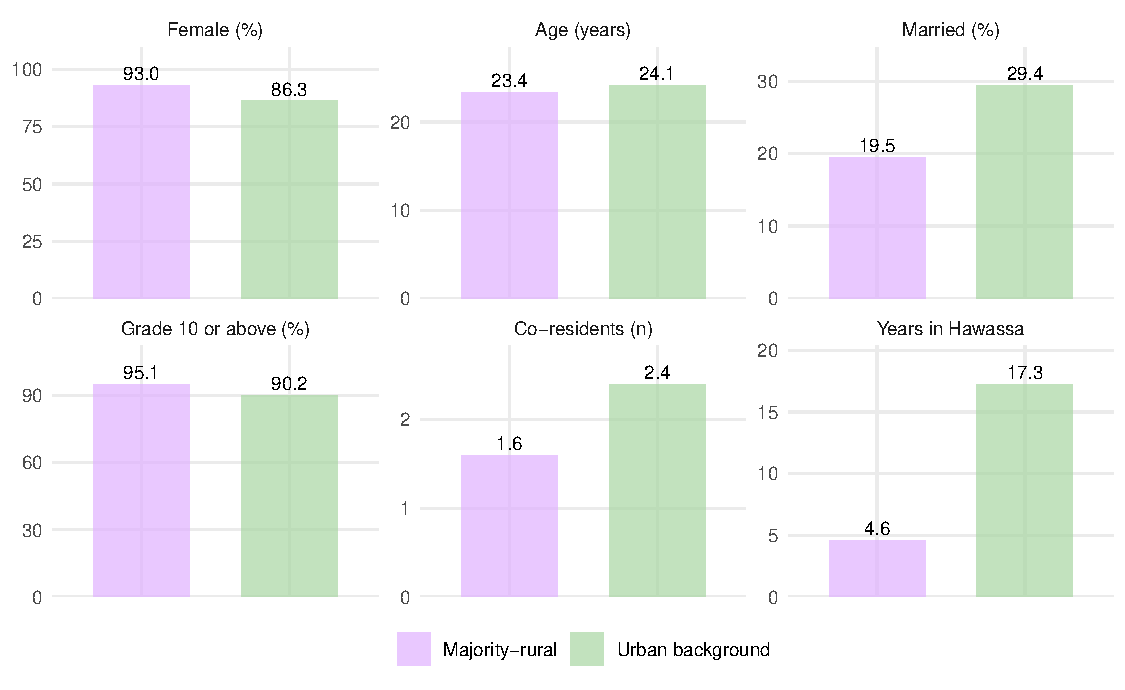
\includegraphics[width=0.8\textwidth]{../figures/fig_setting_demographics}
\fignote{A worker is majority-rural if more than half her life was spent in a rural area.}
\end{figure}

\noindent Workers were interviewed in person shortly after being hired. The median worker was interviewed \pnHireLagMedian{} days after her hire, with \pnHireWithinMonthPct{}\% reached within thirty days and \pnHireWithinTwoMonthPct{}\% within sixty. As mentioned previously, the intention of the design is to observe networks close to their point of formation. \\

\noindent Recruited workers come from a tight regional catchment, with \pnBornSidamaPct{}\% of our sample born in Sidama region, of which Hawassa is the capital (Appendix Figure~\ref{fig:catchment}).  We can infer that most of them are from the Sidama group, the majoritarian ethnicity in the region, a reading consistent with the fluency profile in Figure~\ref{fig:language}. The largest minority, \pnBornWolaytaPct{}\%, comes from Wolayta in the neighbouring South Ethiopia region. It is likely that this concentration has a political history. Hawassa formerly belonged to the multi-ethnic Southern Nations region, until a  referendum calling for Sidama's statehood passed in 2019. The following tensions discouraged workers of other ethnicities from coming to the park \citep{agarwal2026fieldnotes}. \\
\clearpage

\begin{figure}[h!]
\centering
\caption{Speaking fluency in Sidamigna and Amharic}
\label{fig:language}
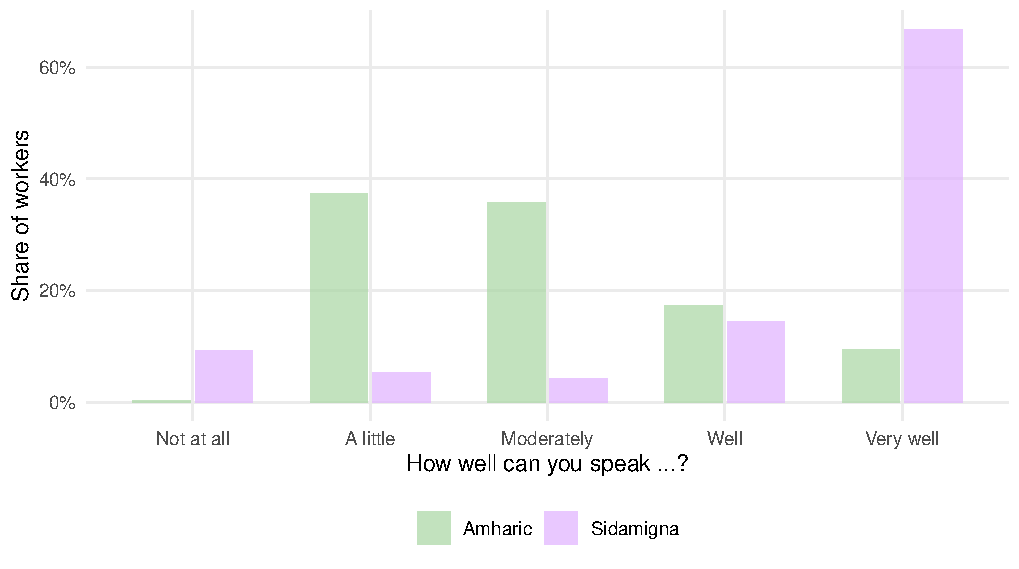
\includegraphics[width=0.8\textwidth]{../figures/fig_setting_language}
\end{figure}

\noindent Of sampled workers, \pnSidamaSpeakPct{}\% speak Sidamigna (the Sidama language, widely spokem in the country side) very well, while only \pnAmharicSpeakPct{}\% speak Amharic (nominally the Ethiopian lingua franca) at least well. Workers from Wolayta and elsewhere speak essentially no Sidamigna, so cross-group communication likely runs through weakly-held Amharic. \\

\noindent Workers all live in Hawassa, and are dispersed across Hawassa’s peri-urban kebeles\footnote{The smallest Ethiopian adminstrative unit, equivalent to a neighbourhood. Other administrative units are Region > Zone > Woreda > Kebele.} rather than concentrated near the park. Indeed, rents in Hawassa are too high relative to factory wages, and the park's own rental compounds are reported to take over half a monthly salary \citep{agarwal2026fieldnotes}. Workers commute by firm-provided bus or on foot. Co-workers feature predominantly as housemates, with \pnLiveCoworkerPct{}\% of workers living with at least one HIP co-worker. Urban-background workers more often live with relatives (Appendix Figure \ref{fig:housing}). \\

\noindent The median worker earns \pnWageMedian{} Birr a month at HIP\footnote{18 US dollars, August 2026 exchange rates}, with an interquartile range of \pnWagePTwentyFive{} to \pnWagePSeventyFive{} Birr (Appendix Table~\ref{tab:livelihoods}). Median household income over the previous three months (including the workers' own earnings, her partner's and any other member's) is \pnHhIncomeMedianThreeMo{} Birr.  The median reservation wage for an outside offer is \pnResvRatioMedian{} times her current wage. This tracks the market, as field informants put non-factory work in Hawassa (such as in services or construction) at around 5{,}000 Birr against 1{,}000-2{,}000 in the factories \citep{agarwal2026fieldnotes}. The worker spent a median of \pnDaysFindJobMedian{} days finding a job at HIP. \\

\noindent People working at HIP cannot live from their income: family transfers to workers are common precisely because the wage does not cover subsistence on its own \citep{agarwal2026fieldnotes}. On average, they are net receivers of financial help. Support comes from outside the factory. Other non-HIP contacts are the most common source,  while the home village follows. Transfers with co-hires exist but are the smallest on both margins. \\
\clearpage

\begin{figure}[h!]
\centering
\caption{Transfers by social group and direction, last 3 months.}
\label{fig:transfers}
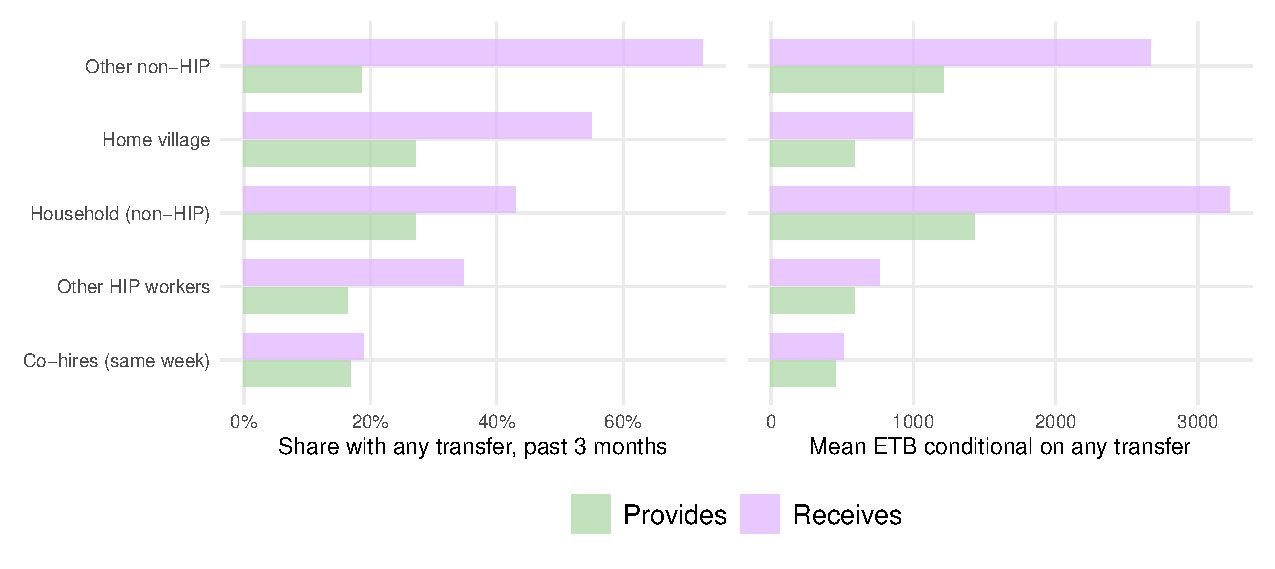
\includegraphics[width=\textwidth]{../figures/fig_setting_transfers}
\end{figure}

\noindent The median worker reports \pnMedNetworkWord{} network members, of which typically one is a co-hire (Figure~\ref{fig:network_size}). Co-hire ties tend to live in the workplace generators, such as breaks, friendship and commuting (Appendix Figure~\ref{fig:generators}). The money generators are answered mainly from the general network. \\

\begin{figure}[h!]
\centering
\caption{Network size per worker, by alter type}
\label{fig:network_size}
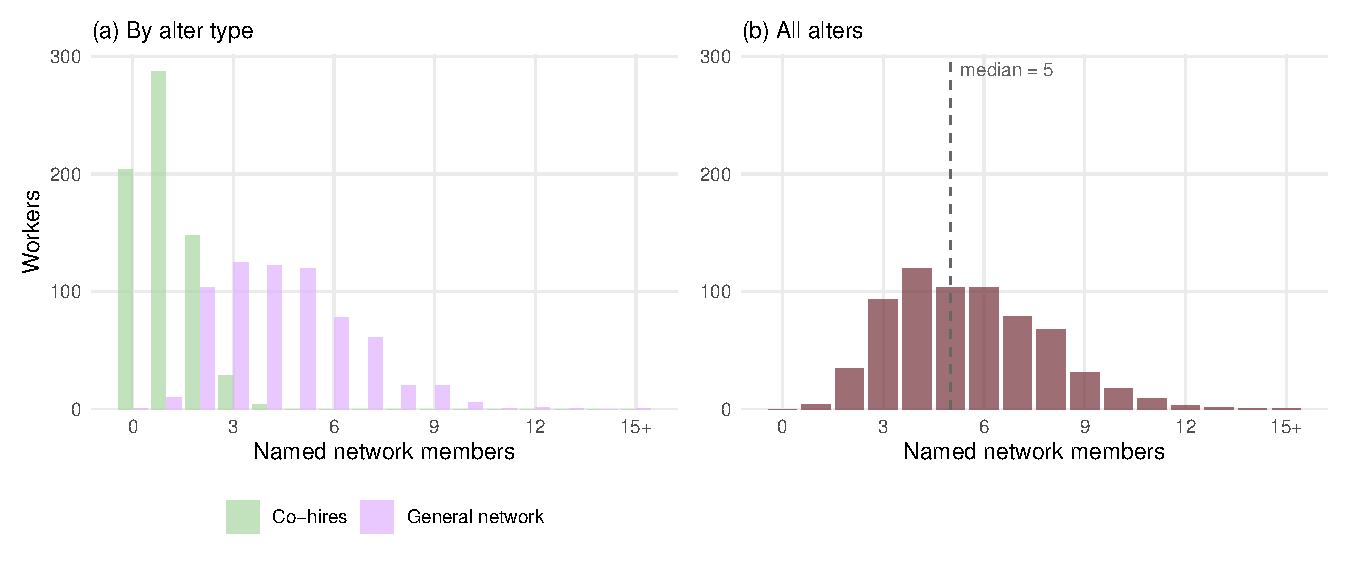
\includegraphics[width=\textwidth]{../figures/fig_setting_network_size}
\end{figure}

\clearpage
\parhead{On the recall of co-hires}

\noindent As mentioned previously, one of the first steps of the survey involves asking the respondent which ones of her co-hires she recalls. The median worker was trained with \pnRecallRosterMedian{} different people and recalled \pnRecallCountMedian{}, a median recall rate of \pnRecallRateMedianPct{}\%. \\

\noindent Of the \pnDyads{} pairs in which both members were themselves surveyed, \pnRecalledDyadPct{}\% are recalled and \pnTiedDyadPct{}\% are named on at least one of the fifteen layers. Given that a worker recalls a co-hire at all, she names her on some layer \pnTiedGivenRecalledPct{}\% of the time. The low tie rate is explained thus by the lack of recall. This suggests that people do not bond much over training. 

\begin{figure}[h!]
\centering
\caption{Recall rate against the number of names shown}
\label{fig:recall_roster}
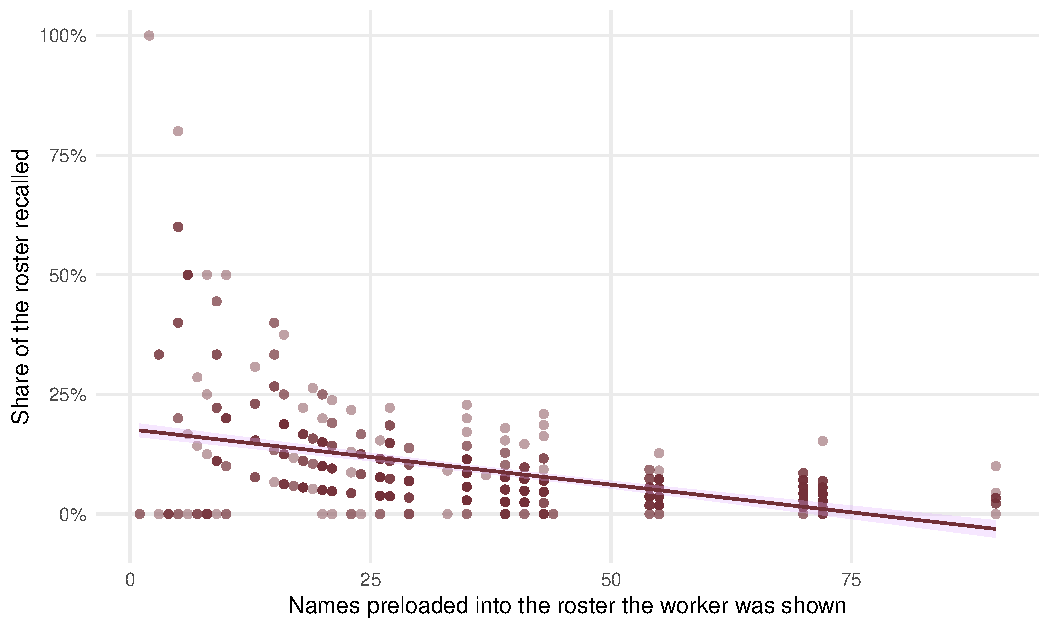
\includegraphics[width=0.8\textwidth]{../figures/fig_setting_recall_by_roster}
\fignote{One point is a worker; the line is the linear fit.}
\end{figure}

\noindent The recall rate falls in roster size, by \pnRecallSlopePerTen{} percentage points per ten additional names (Figure~\ref{fig:recall_roster}; $p = \pnRecallSlopeP{}$, heteroskedasticity-robust). This is driven by the denominator: across quartiles of roster size the median roster grows from \pnRecallRosterQOne{} names to \pnRecallRosterQFour{}, while the mean number recalled goes only from \pnRecallCountQOne{} to \pnRecallCountQFour{}. It appears as respondants have somehow a budget of about \pnRecallCountMedian{} people they can recall.\\

\parhead{On tie reciprocity of co-hires}

\noindent An important concern when working with this type of data is making sure we are recording real ties (and not noise). One way to check for this is what I call reciprocity - if A has nominated B, did B nominate A? On the \pnMutualPairs{} pairs where both workers were surveyed and each appeared on the other's roster, a report by one can be checked against the other. \\

\noindent I expect some relationship layers to be mutual, and other to be more directional. Layers more mutual by nature (\textit{e.g.} commuting together, taking breaks together) reciprocate at \pnRecipReciprocalPct{}\% pooled. Layers such as asking for advice or receiving money reciprocate at \pnRecipDirectionalPct{}\% (Table~\ref{tab:reciprocity}, Figure~\ref{fig:reciprocity}). Co-hire recall itself reciprocates at \pnRecipRecallPct{}\%. 

\begin{table}[h!]
\centering
\caption{Reciprocity by layer}
\label{tab:reciprocity}
\small% GENERATED by "14 descriptives - recall.R" - do not edit by hand.
\begin{tabular}{lrrr}
\textit{layer} & \textit{reported} & \textit{confirmed} & \textit{reciprocity} \\
\dmidrule
\multicolumn{4}{l}{\textit{Expected reciprocal}} \\
\quad Co-hire recall & 1{,}203 & 432 & 36\% \\
\quad Navigate hawassa & 205 & 48 & 23\% \\
\quad Commute & 287 & 98 & 34\% \\
\quad Meet outside work & 209 & 58 & 28\% \\
\quad Call or text & 275 & 82 & 30\% \\
\quad Workplace breaks & 413 & 124 & 30\% \\
\quad Friends & 355 & 110 & 31\% \\
\quad Rosca ekub & 21 & 0 & 0\% \\
\addlinespace
\multicolumn{4}{l}{\textit{Expected directional}} \\
\quad Advice personal decision & 209 & 38 & 18\% \\
\quad Borrow money (in) & 217 & 30 & 14\% \\
\quad Large expenses (in) & 43 & 0 & 0\% \\
\quad Job search & 174 & 26 & 15\% \\
\quad Assistance (in) & 103 & 18 & 18\% \\
\quad Borrow money (out) & 79 & 4 & 5\% \\
\quad Large expenses (out) & 7 & 0 & 0\% \\
\quad Assistance (out) & 22 & 0 & 0\% \\
\bottomrule
\end{tabular}

\fignote{Restricted to the \pnMutualPairs{} pairs in which each worker appeared on the other's roster. \textit{Reciprocity} is \textit{confirmed} over \textit{reported}.}
\end{table}

\begin{figure}[h!]
\centering
\caption{Reciprocity by layer and expected direction}
\label{fig:reciprocity}
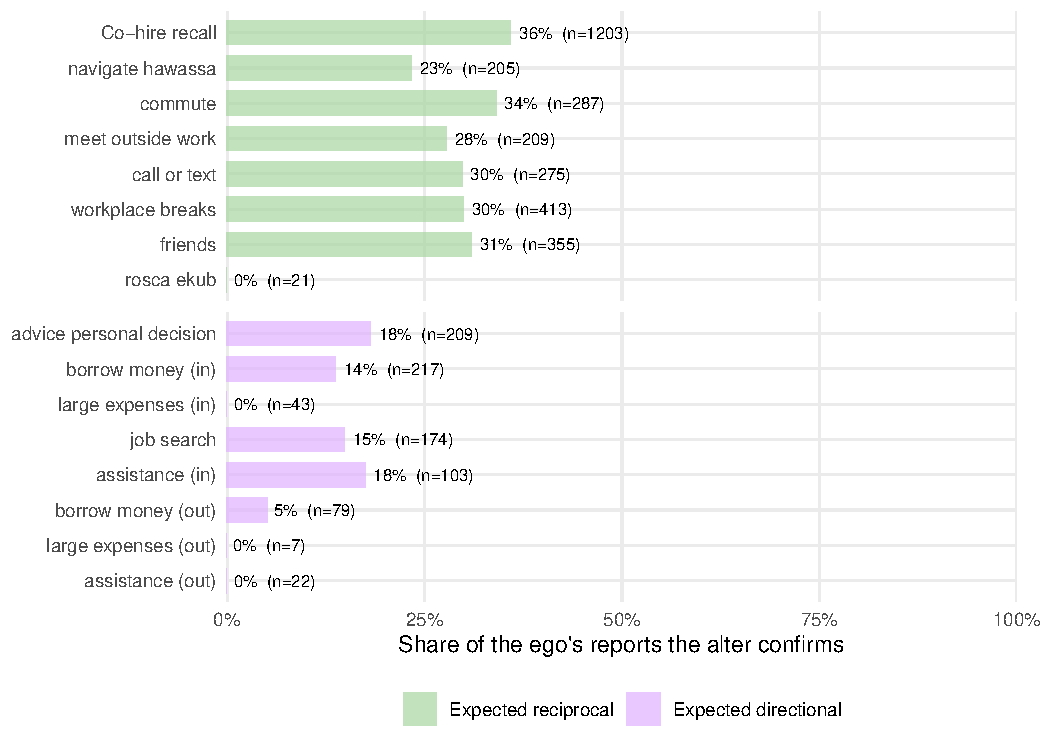
\includegraphics[width=0.85\textwidth]{../figures/fig_setting_reciprocity}
\end{figure}
\clearpage

\noindent Note that risk-sharing layers have low mentions and low reciprocity rates because, as seen in Figure~\ref{fig:transfers}, these are more general network relationships. This sections only looks at co-hires, as it is the only category we can verify. \\

\parhead{On the inheritance of ties}

\noindent Even if this section is descriptive, it starts to document the answer to my questions. Indeed, we can see that network workers report is overwhelmingly inherited. On average, \pnPreHipSharePct{}\% of named alters were known before joining HIP, and \pnPreHipHalfPct{}\% of workers knew at least half of their named network from before entry. The distribution is  more concentrated for urban-background workers than for the majority-rural (Figure~\ref{fig:inherited}). \\

\begin{figure}[h!]
\centering
\caption{Cumulative distribution of pre-HIP share, by background.}
\label{fig:inherited}
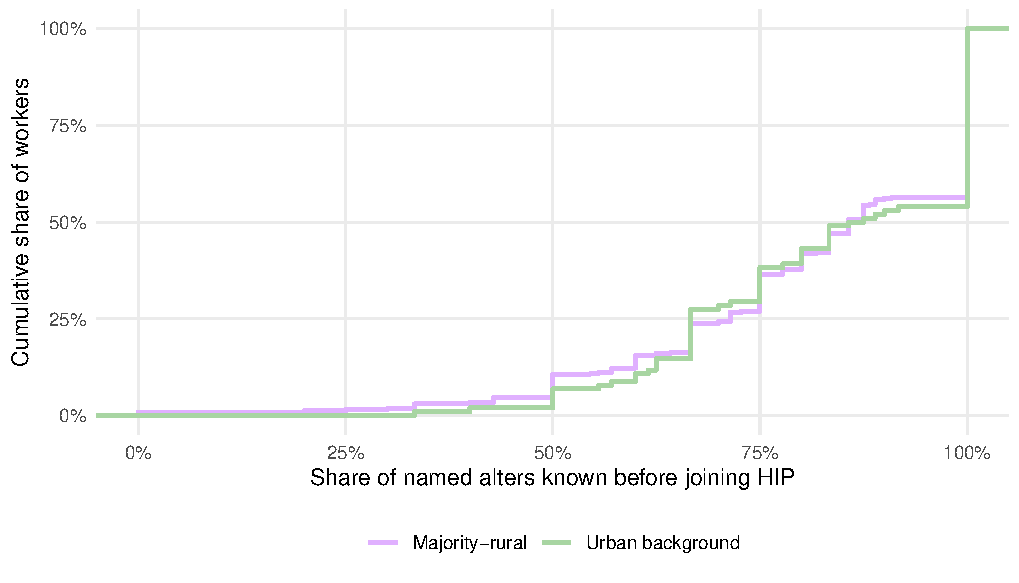
\includegraphics[width=0.8\textwidth]{../figures/fig_setting_inherited}
\end{figure}

\noindent This is not only driven by the general network, as we may expect\footnote{As a reminder, co-hire ties are between two workers, whereas general-network alters are described only by the respondent and are mostly not HIP employees.}.  About \pnTieCohireInheritedPct{}\% co-hire ties are inherited (\pnTieCohireInherited{} of them), against \pnTieGnInheritedPct{}\% of general-network ties (\pnTieGnInherited{}). Inherited co-hire ties are \pnTieCohireFriendPct{}\% friendships, against \pnTieCohireKinPct{}\% kin. In the general network the split is \pnTieGnKinPct{}\% kin against \pnTieGnFriendPct{}\% friends. It appears as the inherited general network is the origin community, while the inherited part of the co-hire network is a thinner and more geographically dispersed set of friendships (Table~\ref{tab:tie_composition}). \\

\begin{table}[h!]
\centering
\caption{Composition of inherited ties, by roster}
\label{tab:tie_composition}
% GENERATED by "16 descriptives - ties and dyads.R" - do not edit by hand.
\begin{tabular}{lrrr}
& \textit{ties} & \textit{\% of inherited} & \textit{\% co-villager} \\
\dmidrule
\multicolumn{4}{l}{\textit{Co-hire ties}} \\
Kin & 37 & 12.2 & 55.6 \\
Friends & 231 & 76.2 & 20.6 \\
Acquaintances & 35 & 11.6 & 9.1 \\
\midrule
\multicolumn{4}{l}{\textit{General network}} \\
Kin & 1{,}450 & 52.2 & 86.9 \\
Friends & 1{,}206 & 43.4 & 48.3 \\
Acquaintances & 122 & 4.4 & 25.6 \\
\bottomrule
\end{tabular}

\fignote{One observation is an inherited tie; shares are within roster. \textit{Kin} covers all family codes (1--6). \textit{\% co-villager} is the share born in the worker's own woreda, over ties with a usable origin code.}
\end{table}

\noindent On a side note, it appears as information about the job travels to the general network. Even if \pnJobInfoNonePct{}\% of the analysis sample (\pnJobInfoNone{} of \pnAnalysisN{} workers) report that they gathered information about jobs in the Park from no one, the remaining \pnJobInfoEgos{} name \pnJobInfoTies{} general-network informants. These informants are \pnJobInfoFriendPct{}\% friends and \pnJobInfoKinPct{}\% kin. \\

\FloatBarrier
\parhead{On the depth and multiplexing of ties}

\noindent As suggested before, a relationship is rarely one thing at a time. The friend you commute with may also be the one you confide in, and your landlord might very well be your partner. This is dubbed a multiplex network. In our sample, \pnMuxCohireTwoPct{}\% of co-hire ties span at least two layers and \pnMuxCohireSixPct{}\% span six or more. For general-network ties,  \pnMuxGnTwoPct{}\% are multiplex and \pnMuxGnSixPct{}\% span six or more layers (Figure \ref{fig:multiplex}). \\

\begin{figure}[h!]
\centering
\caption{Number of ties each alter appears in, by type}
\label{fig:multiplex}
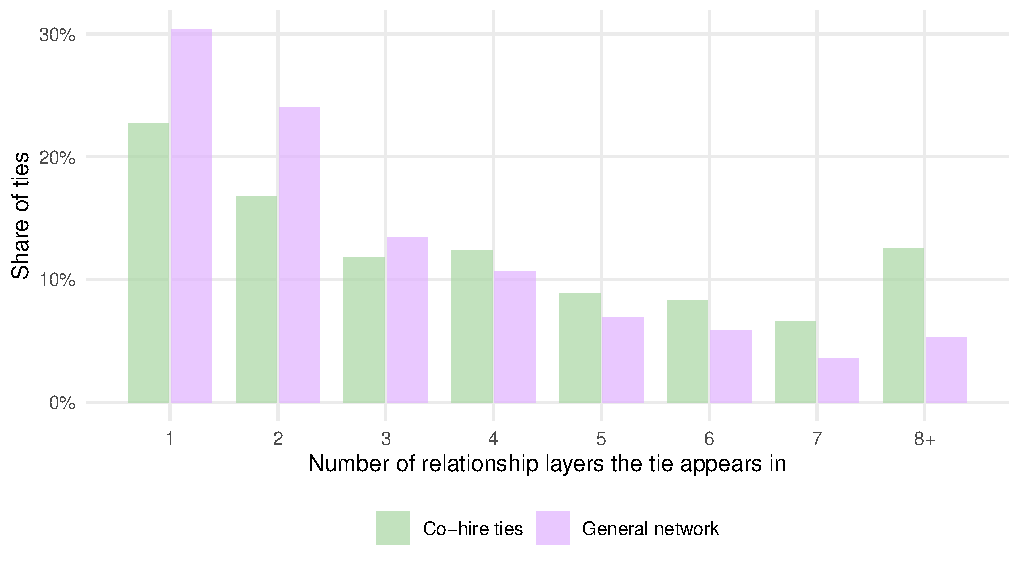
\includegraphics[width=0.8\textwidth]{../figures/fig_setting_multiplex}\end{figure}
\FloatBarrier

\noindent The question becomes which ties are grouped together, or which type of relationships are usually multiplex. Figure~\ref{fig:cooc} analyses the fifteen layers pairwise. A cell is the probability that a tie already carrying the row layer also carries the column layer. \\

\begin{figure}[h!]
\centering
\caption{Which relationship layers travel together? Conditional Probability}
\label{fig:cooc}
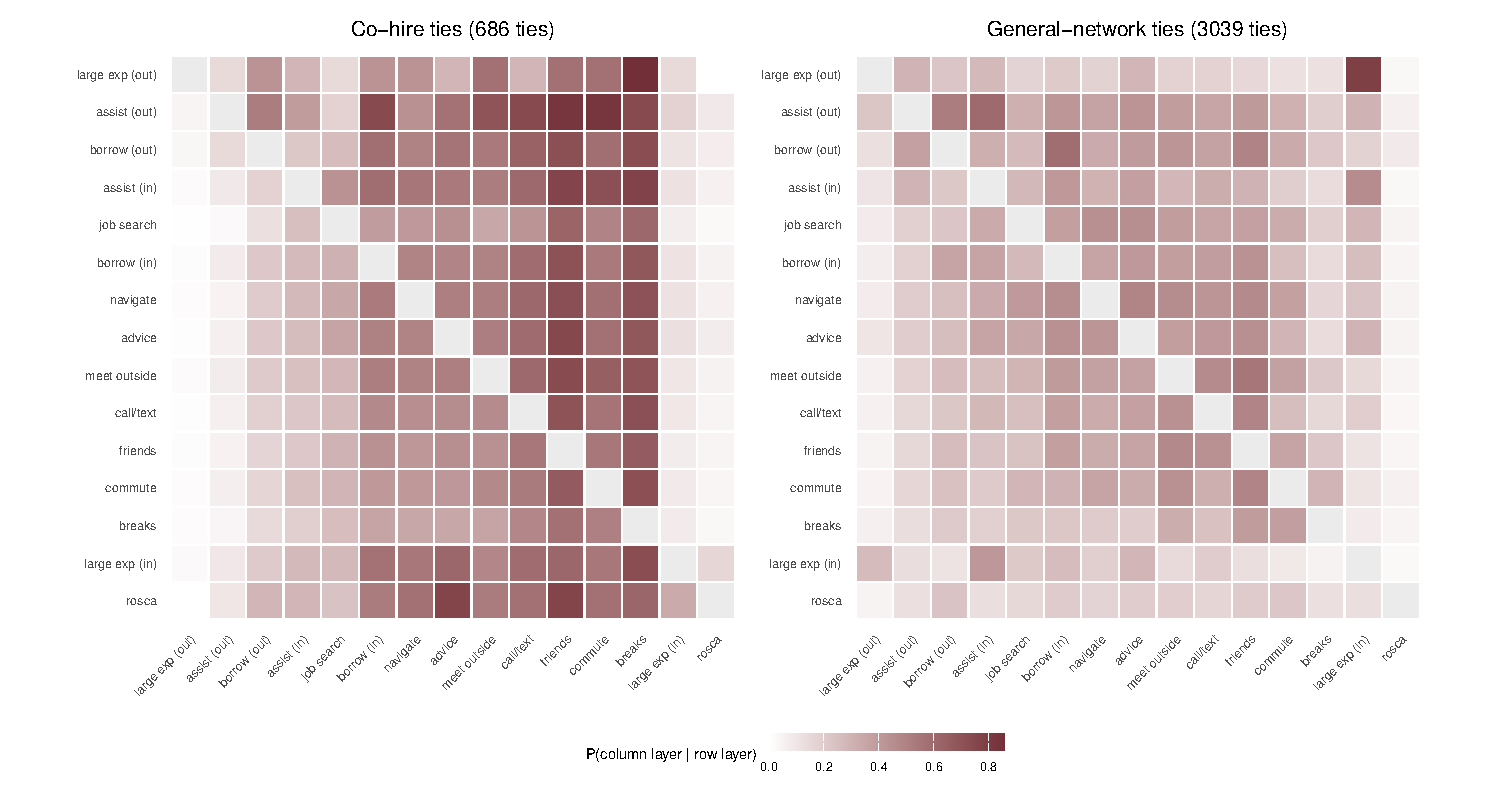
\includegraphics[width=\textwidth]{../figures/fig_setting_layer_cooc_cond}
\fignote{A cell is the share of ties carrying the row layer that also carry the column layer, so the matrix is asymmetric. \textit{large expenses (out)}, \textit{Rosca} and \textit{large expenses (in)} rest on \pnThinLargeExpOut{}, \pnThinRosca{} and \pnThinLargeExpIn{} ties; their rows read dark only because those \pnThinLargeExpOutWord{} ties are dense ones.}
\end{figure}
\FloatBarrier
\noindent Co-hire relationships are thinner than the general network, which makes sense since they are no older than the worker's tenure at HIP. Among co-hire ties, a tie carrying one layer associated to companionship (commuting, breaks, friendship, meeting outside work, calling) carries another given companionship layer with probability \pnCondCompCohire{} (\pnCondCompGn{} for the general network), but carries any given risk-sharing outflow with probability \pnCondOutCohire{} (\pnCondOutGn{} for the general network). Only \pnAnyOutCohirePct{}\% of co-hire ties carry some risk-sharing outflow overall (\pnAnyOutGnPct{} for the general network), and \pnAnyOutCommuteCohirePct{}\% of those that carry commuting do (\pnAnyOutCommuteGnPct{} for the general network). \\

\parhead{Observations}

\noindent We have now a clear picture of the environment these people evolve in. People remain tied to their origin community and inherit \pnTieCohireInheritedPct{}\% of the colleagues they name at work. They do not recall many people from their trainings, and form new ties for company rather than for risk-sharing. A month after arriving, her usable network is essentially the one she brought with her. \\

\noindent The set-up that follows in the next section is minimal. Its purpose is to show that the aforementioned four channels can be thought as parameters of a same model. It allows me to identify what I can try to estimate. 

